%\setchapterimage{Header_Peugeot.jpg}
\setchapterpreamble[u]{\margintoc}
%\setcounter{chapter}{1}

\chapter{Modélisation géométrique -- Lois entrées-sorties}

\marginnote[8cm]{
%\UPSTIcompetence[2]{B2-14}
%\UPSTIcompetence[2]{C2-03}
}

%\begin{marginfigure}
%\includegraphics[width=4cm]{newton}%images/prot_01
% \capture{Isaac Newton -- 1643 - 1727.}
% \end{marginfigure}
% 
% 
\section{Modélisation et paramétrage des systèmes mécaniques}
\begin{methode}[Modélisation d'un système mécanique réel]

Pour modéliser un système mécanique réel (en TP par exemple) il faut : 
\begin{itemize}
\item identifier les classes d'équivalence cinématique, c'est-à-dire tous les ensembles de pièces reliés entre elles par des liaisons encastrement;
\item identifier les surfaces de contact entre les classes d'équivalence;
\item associer une liaison cinématique aux surfaces de contact;
\item tracer les liaisons en utilisant une couleur par classe d'équivalence et respectant leur positionnement relatif;
\item relier les liaisons de manière filaire;
\item indiquer le bâti, les centres de liaisons et la numérotation des classes d'équivalence.
\end{itemize}
\end{methode}

\marginnote{
Par usage, nous associerons une lettre grecque à un paramètre variable et une lettre romane à une dimension fixe. Cela permet de repérer plus facilement quelles sont les variables temporelles lors de calcul de dérivées.}

\begin{methode}[Paramétrage d'un mécanisme cinématique]
Pour paramétrer un mécanisme, il faut associer un repère à chaque classe d'équivalence, une constante à chaque dimension fixe (pour une même classe d'équivalence) et une variable à chaque degré de mobilité de liaison (entre deux classes d'équivalence). 
\begin{itemize}
\item si la mobilité est une translation, on définit un paramètre variable entre deux points selon une seule direction (la direction de la translation);
\item si la mobilité est une rotation il faut définir l'axe de rotation et l'angle variable en précisant la figure de changement de base.
\end{itemize}
%\begin{rem}
%\end{rem}
\end{methode}

\begin{defi}[Graphe de structure -- Chaînes]

Graphe qui permet d'avoir une vue d'ensemble du mécanisme :
\begin{itemize}
\item les classes d'équivalences sont schématisées par des cercles avec un repère (celui défini précédemment);
\item les liaisons sont schématisées par des traits qui relient les cercles.
\end{itemize}

On définit 3 types de chaînes :
\begin{center}
\begin{tabular}{ccc}
Les chaînes ouvertes & Les chaînes fermées & Les chaînes complexes \\
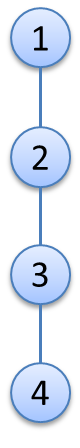
\includegraphics[height=3cm]{co.png}
&
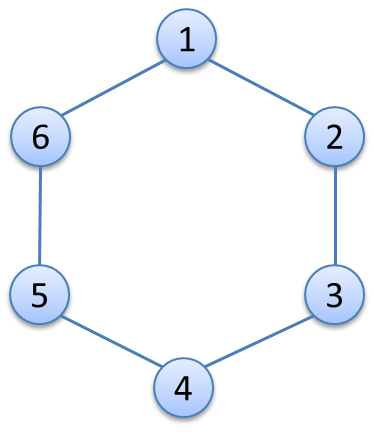
\includegraphics[height=3cm]{cf.png}
&
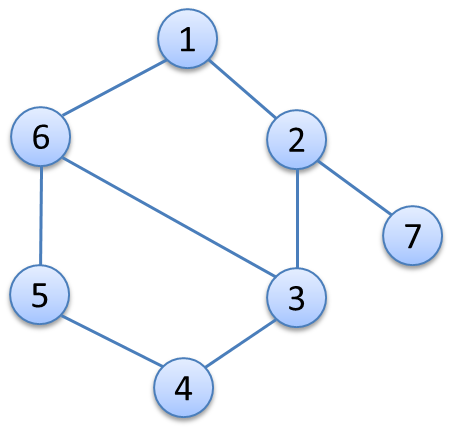
\includegraphics[height=3cm]{cc.png}\\
\end{tabular}
\end{center}
\end{defi}


\section{Résolution des lois entrée--sortie}


\begin{methode}
\textbf{Calcul de la loi Entrée -- Sortie dans une chaîne de solides fermée}

Un système se présentant sous forme d'une chaîne de solide fermée a pour but de transformer un mouvement. On s'intéresse alors pour cela à la relation cinématique liant le mouvement d'entrée du système et le mouvement de sortie. On écrit pour cela une \textbf{fermeture de chaîne géométrique}. Pour cela :
\begin{enumerate}
\item paramétrer le mécanisme;
\item identifier la grandeur d'entrée et de sortie;
\item à l'aide du théorème de Chasles, exprimer le vecteur nul en fonction des vecteurs liant le centre de chacune des liaisons;
\item projeter la relation vectorielle sur une des bases;
\item combiner les relations pour exprimer la sortie en fonction de l'entrée;
\item dériver si besoin pour avoir le lien entre les vitesses. 
\end{enumerate}
\end{methode}


\begin{methode}
\textbf{Méthodes pour manipuler les systèmes équations :} 
\begin{enumerate}
\item Pour supprimer une longueur $\lambda$ : on met les deux équations sous la forme $\lambda =$ et on fait le rapport des deux équations.
\item Pour supprimer l'angle $\varphi$ : on met une équation sous la forme $\cos\varphi = $ et la seconde sous la forme $\sin\varphi = $ et on utilise la relation $\cos^2\varphi +\sin^2\varphi =1 $.
\item Dans d'autres cas, on peut avoir à utiliser l'expression de la tangente.
\end{enumerate}
\end{methode}


\begin{methode}[Autre idée pour calculer la loi Entrée -- Sortie dans une chaîne de solides fermée]
Dans certains mécanismes, on peut observer que deux vecteurs sont toujours orthogonaux. En utilisant le fait que le produit scalaire entre ces deux vecteurs est nul puis en projetant les vecteurs dans une même base puis en réalisant le calcul, il est possible de déterminer une loi entrée-sortie.
\end{methode}
%\end{document}


